% This is "sig-alternate.tex" V2.1 April 2013
% This file should be compiled with V2.5 of "sig-alternate.cls" May 2012
%
% This example file demonstrates the use of the 'sig-alternate.cls'
% V2.5 LaTeX2e document class file. It is for those submitting
% articles to ACM Conference Proceedings WHO DO NOT WISH TO
% STRICTLY ADHERE TO THE SIGS (PUBS-BOARD-ENDORSED) STYLE.
% The 'sig-alternate.cls' file will produce a similar-looking,
% albeit, 'tighter' paper resulting in, invariably, fewer pages.
%
% ----------------------------------------------------------------------------------------------------------------
% This .tex file (and associated .cls V2.5) produces:
%       1) The Permission Statement
%       2) The Conference (location) Info information
%       3) The Copyright Line with ACM data
%       4) NO page numbers
%
% as against the acm_proc_article-sp.cls file which
% DOES NOT produce 1) thru' 3) above.
%
% Using 'sig-alternate.cls' you have control, however, from within
% the source .tex file, over both the CopyrightYear
% (defaulted to 200X) and the ACM Copyright Data
% (defaulted to X-XXXXX-XX-X/XX/XX).
% e.g.
% \CopyrightYear{2007} will cause 2007 to appear in the copyright line.
% \crdata{0-12345-67-8/90/12} will cause 0-12345-67-8/90/12 to appear in the copyright line.
%
% ---------------------------------------------------------------------------------------------------------------
% This .tex source is an example which *does* use
% the .bib file (from which the .bbl file % is produced).
% REMEMBER HOWEVER: After having produced the .bbl file,
% and prior to final submission, you *NEED* to 'insert'
% your .bbl file into your source .tex file so as to provide
% ONE 'self-contained' source file.
%
% ================= IF YOU HAVE QUESTIONS =======================
% Questions regarding the SIGS styles, SIGS policies and
% procedures, Conferences etc. should be sent to
% Adrienne Griscti (griscti@acm.org)
%
% Technical questions _only_ to
% Gerald Murray (murray@hq.acm.org)
% ===============================================================
%
% For tracking purposes - this is V2.0 - May 2012

\documentclass{sig-alternate-05-2015}

\usepackage{xcolor}
\usepackage{amsmath}
\usepackage{algorithm}
\usepackage[noend]{algpseudocode}
\makeatletter
\def\BState{\State\hskip-\ALG@thistlm}
\makeatother

\newcommand\TODO[1]{\textcolor{red}{#1}}
\newcommand{\lucenequery}[1]{\vspace{1mm}\texttt{#1}\vspace{1mm}}

\begin{document}

% Copyright
\setcopyright{acmcopyright}
%\setcopyright{acmlicensed}
%\setcopyright{rightsretained}
%\setcopyright{usgov}
%\setcopyright{usgovmixed}
%\setcopyright{cagov}
%\setcopyright{cagovmixed}


% DOI
\doi{10.475/123_4}

% ISBN
\isbn{123-4567-24-567/08/06}

%Conference
\conferenceinfo{PLDI '13}{June 16--19, 2013, Seattle, WA, USA}

\acmPrice{\$15.00}

%
% --- Author Metadata here ---
\conferenceinfo{KDD}{'17 Halifax, Nova Scotia, Canada}
%\CopyrightYear{2007} % Allows default copyright year (20XX) to be over-ridden - IF NEED BE.
%\crdata{0-12345-67-8/90/01}  % Allows default copyright data (0-89791-88-6/97/05) to be over-ridden - IF NEED BE.
% --- End of Author Metadata ---

\title{Latency Reduction via Decision Tree Based Query Construction}
% You need the command \numberofauthors to handle the 'placement
% and alignment' of the authors beneath the title.
%
% For aesthetic reasons, we recommend 'three authors at a time'
% i.e. three 'name/affiliation blocks' be placed beneath the title.
%
% NOTE: You are NOT restricted in how many 'rows' of
% "name/affiliations" may appear. We just ask that you restrict
% the number of 'columns' to three.
%
% Because of the available 'opening page real-estate'
% we ask you to refrain from putting more than six authors
% (two rows with three columns) beneath the article title.
% More than six makes the first-page appear very cluttered indeed.
%
% Use the \alignauthor commands to handle the names
% and affiliations for an 'aesthetic maximum' of six authors.
% Add names, affiliations, addresses for
% the seventh etc. author(s) as the argument for the
% \additionalauthors command.
% These 'additional authors' will be output/set for you
% without further effort on your part as the last section in
% the body of your article BEFORE References or any Appendices.
\numberofauthors{1} 
\author{
\alignauthor Aman Grover, Dhruv Arya, Ganesh Venkataraman \\
\affaddr{LinkedIn Corporation} \\ \affaddr{Sunnyvale, CA, USA} \\
\email{\{agrover,darya,ghvenkat\}@linkedin.com}
}
% There's nothing stopping you putting the seventh, eighth, etc.
% author on the opening page (as the 'third row') but we ask,
% for aesthetic reasons that you place these 'additional authors'
% in the \additional authors block, viz.
\additionalauthors{Additional authors: John Smith (The Th{\o}rv{\"a}ld Group,
email: {\texttt{jsmith@affiliation.org}}) and Julius P.~Kumquat
(The Kumquat Consortium, email: {\texttt{jpkumquat@consortium.net}}).}
\date{30 July 1999}

% Just remember to make sure that the TOTAL number of authors
% is the number that will appear on the first page PLUS the
% number that will appear in the \additionalauthors section.

\maketitle
\begin{abstract}
LinkedIn as a professional network serves the career needs of 450 Million plus members. 
The task of job recommendation system is to find the suitable job among a corpus of several million jobs and serve this in real time under tight latency constraints. 
Job search involves finding suitable job listings given a user, query and
context.  Typical scoring function for both search and recommendations 
involves evaluating a function that matches various fields in the job description 
with various fields in the member profile.
This in turn translates to evaluating a function with several thousands of features to get the right ranking. 
In recommendations, evaluating all the jobs in the corpus for all members is not possible given the latency constraints. 
On the other hand, reducing the candidate set could 
potentially involve loss of relevant jobs. 
This work provides a novel way of improving the candidate jobs for the job seeker without hurting the overall relevance of the product. 
We propose a novel way to model the underlying complex ranking function with a
decision tree. The variable within the branching of the decision tree would be
candidate query clauses. We developed an offline framework which
evaluates the quality of the decision tree with respect to latency and recall.
We tested the approach on job search and recommendations on LinkedIn and A/B tests show significant improvements in member engagement and latency. 
Our techniques helped reduce job search latency by over {\bf 67\%} and our
recommendations latency by over {\bf 55\%}.
{\bf As of writing the approach powers all of job search and recommendations on LinkedIn.} 

\end{abstract}

%
% The code below should be generated by the tool at
% http://dl.acm.org/ccs.cfm
% Please copy and paste the code instead of the example below. 
%
\begin{CCSXML}
<ccs2012>
 <concept>
  <concept_id>10010520.10010553.10010562</concept_id>
  <concept_desc>Information retrieval~Document filtering</concept_desc>
  <concept_desc>Recommender Systems~Query Reformulation</concept_desc>
  <concept_desc>Machine Learning~Decision Trees</concept_desc>
  <concept_significance>500</concept_significance>
 </concept>
 <concept>
  <concept_id>10010520.10010575.10010755</concept_id>
  <concept_desc>Computer systems organization~Redundancy</concept_desc>
  <concept_significance>300</concept_significance>
 </concept>
 <concept>
  <concept_id>10010520.10010553.10010554</concept_id>
  <concept_desc>Computer systems organization~Robotics</concept_desc>
  <concept_significance>100</concept_significance>
 </concept>
 <concept>
  <concept_id>10003033.10003083.10003095</concept_id>
  <concept_desc>Networks~Network reliability</concept_desc>
  <concept_significance>100</concept_significance>
 </concept>
</ccs2012>  
\end{CCSXML}

\ccsdesc[500]{Computer systems organization~Embedded systems}
\ccsdesc[300]{Computer systems organization~Redundancy}
\ccsdesc{Computer systems organization~Robotics}
\ccsdesc[100]{Networks~Network reliability}


%
% End generated code
%

%
%  Use this command to print the description
%
\printccsdesc

% We no longer use \terms command
%\terms{Theory}

\keywords{Information Retrieval, Personalized Search, Recommender Systems}


% end the environment with {table*}, NOTE not {table}!
\section{Introduction}
The jobs ecosystem in LinkedIn powers the career needs of 450 Million plus
professionals around the world. The two main means of finding a job via
LinkedIn are through search and recommendations. Traditional information
retrieval involves matching and scoring a set of documents given query.
Personalized search involves scoring documents given query and {\bf user}~\cite{liget}.  
Both search and recommendations pose unique set of constraints on quality and
latency.

LinkedIn job search and recommendations are used in different parts of the
ecosystem with different types of constraints. 
Figures~[\ref{fig:jymbii-jobs-home}] and~[\ref{fig:jymbii-in-feed}] show the
use case for jobs recommendations in LinkedIn jobs home and LinkedIn feed (home
page) respectively.
The LinkedIn
feed~\cite{agarwal2015personalizing} personalizes the experience by merging
different sources of information including posts, comments, news articles and
jobs. Each of these sources (including job recommendations) must respond with
very tight SLA (Service Level Agreements, usually latency constraints imposed
by the callers of a service)s in order for the home page or the app to be responsive.
In job recommendations, there is no explicit query to filter the results.
The underlying recommendations model is deeply personalized with per member and
per job coefficients. Such personalization helps us achieve very high
relevancy~\cite{zhang2016glmix}. Scoring all possible jobs for each member in
this complex model would be prohibitively expensive and will certainly not meet
our SLA requirements. At the same time, scoring very few documents would result
in loss of relevance. 

Job search has similar issues as well. While search has an explicit query,
sometimes the query can be way too broad (example: {\it marketing}).
These broad queries match several millions of jobs and ranking all of them
would not meet our latency requirements.
There are several such head queries ({\it marketing, sales}) which exhibit
similar characteristics.
In this case we
could leverage information in the members profile to bias the query towards
particular jobs he/she may be interested in.

One common way of handling too many matching documents is to pass through
multiple levels of rankers. The ranker closest to the retrieval stage is coarse
and biases it's decision towards recall and not precision. But, as we move to
higher levels, we move on to more complex rankers which take more time, but
also rank fewer documents. In this regard, we generally separate out the
search/recommendations flow into two steps pre-retrieval and post retrieval.
Pre retrieval involves constructing the query based on both the explicit query
from user as well as personalization added on top of it and post retrieval
involves going through multiple layers of ranking. The post retrieval ranking
for both search and recommendations is well studied~\cite{liu2009learning}. 

The objective of query construction is to formulate a query to our retrieval
engine such that we minimize the number of documents ranked (direct impact on
latency) while making sure we score the relevance documents. In this work we
propose a decision tree based approach towards query construction that meets the
aforementioned objective. The key contribution of the work includes: 
\begin{enumerate}
        \item We convert the query construction problem into a decision tree
            problem with branches in the tree corresponding to query clauses 
            and show that such a formulation scales for very large number of features. 
            We show that such a formulation can have a huge impact on latency
            without affecting quality of the results - all at LinkedIn scale.
        \item We propose an offline replay mechanism which does a true
            evaluation of the underlying ranking metric while evaluating gain
            in latency. It also increases the experimentation velocity by near
            accurate reproduction of production behavior and reduces number of
            A/B tests needed with live traffic.
        \item The framework is generic across search and recommendations so
            long as the underlying retrieval is based on an inverted index.
\end{enumerate}
The techniques described in this work are all in production. In job search it
resulted in p99 (worst 1\% of the queries) latency reduction of {\bf 67\%} 
and in jobs recommendations, we show a p99 latency reduction of {\bf 55.96\%}. While
p99 queries are more important on an operational perspective, we also show
significant reduction in latency for median case as well. While we did not
explicitly target quality metrics, we did find a {\bf 3.5\%} improvement in job
application as a result of this approach. We attribute this improvement mainly
due to reduction in timeouts from our callers (due to improved latency). All
results shown were obtained by online A/B testing. As of writing this paper, 
the techniques described in this work power all of job search and
recommendations at LinkedIn.


\begin{figure}
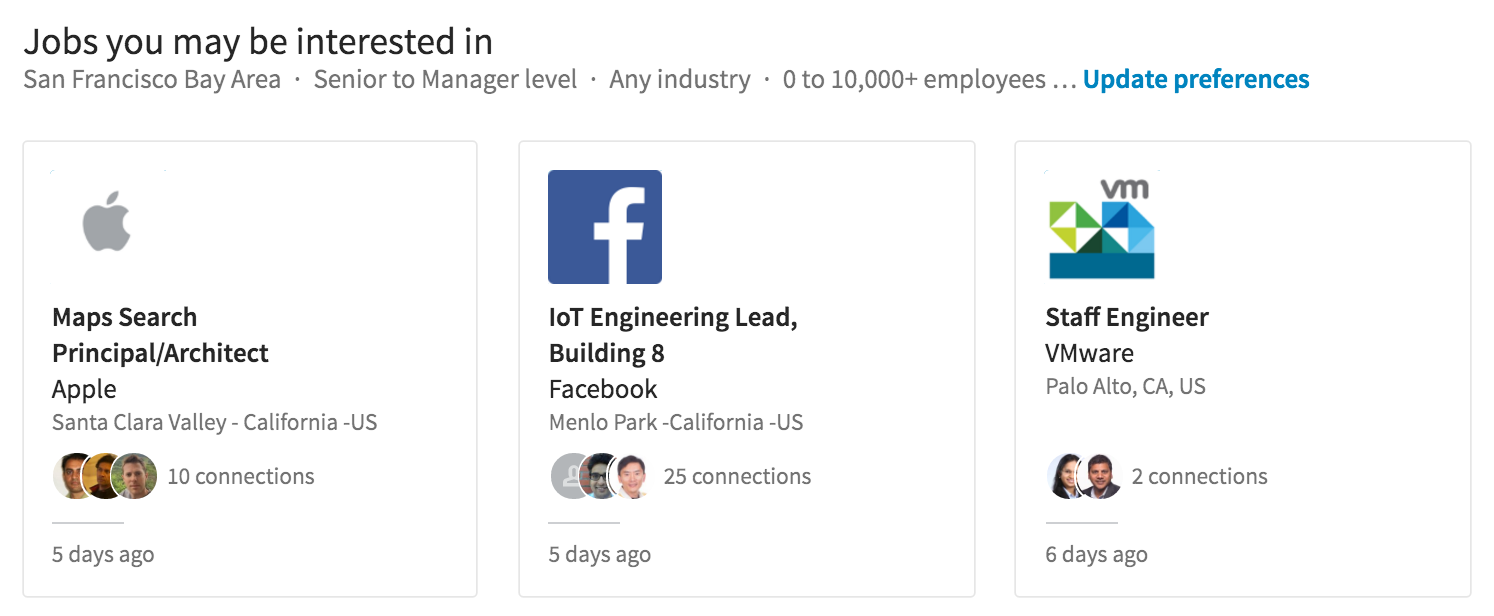
\includegraphics[width=\linewidth,height=\textheight,keepaspectratio]{jymbii.png}
\caption{Jobs recommendations in jobs homepage}
\label{fig:jymbii-jobs-home}
\end{figure}

\begin{figure}
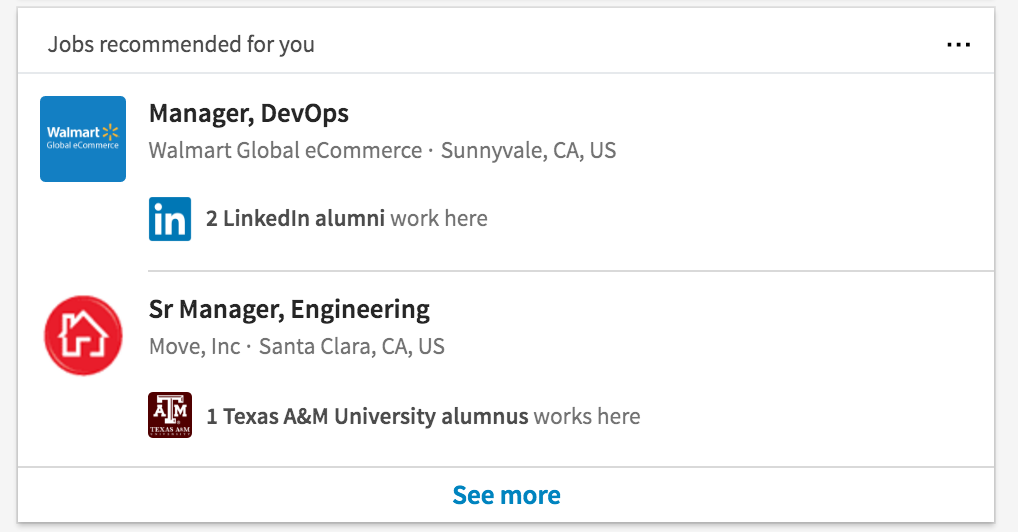
\includegraphics[width=\linewidth,height=\textheight,keepaspectratio]{jymbii-in-feed.png}
\caption{Jobs recommendations in LinkedIn feed}
\label{fig:jymbii-in-feed}
\end{figure}

\section{Related Work}
Query formulation is a well-studied area in Information Retrieval (IR). For
most part, query optimization deals with reducing latency. It also enables use
of more complex/time consuming ranker with fewer number of documents. 
~\cite{broder2003efficient} formally introduces the concept of a WAND (weighted AND) operator which has since
then been extensively used in large scale search systems including LinkedIn.
The WAND operator requires weights and ~\cite{broder2003efficient} proposes
tf-idf based heuristics to tune those weights. Search systems organized in
terms of inverted index ~\cite{goel2009predictive}. For inverted index based
search systems, a common technique used to speed up retrieval is the use of
early termination~\cite{anh2001vector,yan2010efficient,zhang2010revisiting}.
Use of early termination requires that the posting list 
is ordered in such a way that the highest quality document is
placed first. Note that this quality is dependent only on the document and not
the query or the user. This score computed on a per document basis is often
referred to as ``static rank''. 
Various techniques used for computing suitable
static rank includes term frequencies~\cite{persin1996filtered} or the more
popular pagerank~\cite{brin2007anatomy}.
Commonly used scores include within-document term frequencies~\cite{persin1996filtered},
or some notion of document quality or popularity~\cite{brin2007anatomy}.

The authors in~\cite{agarwal2012fast} develop a two-pass approach to ranking. The first pass
retrieves the top-k documents using approximate ranking. The second pass uses a
more accurate model. The document and items are represented in a vector space.
The first state ranking leverages this vector space representation to retrieve
a limited set of documents. This gives more time for the second pass to work on
a more accurate model. 
The authors in~\cite{covington2016deep} construct a neural network based candidate
selection for YouTube recommendations. In this work, the
number of videos to be ranked is reduced to a few hundred's by converting the
recommendation problem into an extreme multi class classification problem. A
high dimensional embedding of each document and item (in this case user and videos) 
is learned using neural networks. A nearest neighbor search is executed in real
time in this high dimensional space to retrieve the top N documents.
The authors in~\cite{aphi2004learning} propose a way to learn Boolean queries in
such a way that they are manageable by humans. Such queries are then used as
filters. 

The work closest to our existing work ~\cite{borisyuk2016casmos} develop a
framework to prune irrelevant documents and retrieve documents that are likely
to be in the top-k results of the query. This is done by training a constrained
feature selection algorithm to learn positive weights for feature combinations
of the weighted candidate query. Our approach while using the same retrieval
engine differs in the following aspects:
\begin{enumerate}
        \item We propose a decision tree based framework to come up directly
            with query clauses. 
        \item We develop an offline replay framework which accurately estimates
            the differences between constrained query formulation vs retrieving
            all documents. ~\cite{borisyuk2016casmos} uses AUC as evaluation.
            AUC is a classification metric while the underlying problem we are
            trying to model is a ranking problem. Pointwise metrics (like AUC)
            are shown to be less accurate~\cite{xia2008listwise,
            liu2009learning}. Since our replay framework models production
            queries on a production index, it reduces the number of iterations
            needed for online A/B testing.
        \item ~\cite{borisyuk2016casmos} does not make use of retrieval
            operators like early termination and suitable static rank. Getting
            a good representative static rank can reduce the latency
            significantly.
\end{enumerate}



\section{Problem Formulation}
Let
\begin{itemize}
    \item $EQ$ represent the explicit user query. In search $EQ$ represents the
        search term and in recommendations $EQ$ is empty.
    \item $U$ represent set of user attributes in the profile. Example -
        current company, current title etc.
    \item $C$ represent the context. This may include past job searches,
        job applies, jobs views etc.
    \item $D(q)$ represents the set of document retrieved from inverted index
        for a given query $q$. $|D(q)|$ represents it's cardinality.
    %\item $M$ represent the set of all documents that match the users explicit
    %    query $EQ$. In recommender systems, $M$
    %    could include all documents in the index. In search, it could be more
    %    restrictive in the presence of an explicit query.
    \item $k$ represent the top documents required to be shown to the user and
        $M$ represent the total number of documents that match the query.
        Typically $k << |M|$.
    \item $R_f(d, k)$ represent the underlying ranking function which generates
        top k documents from document set $d$.  

\end{itemize}
The ranking function takes a (user, query, document) tuple and converts it into a score. Our
ranking function is highly personalized using per member and per job
coefficients. This work doesn't touch the ranking function but modifies the query. 
Interested reader may refer to ~\cite{zhang2016glmix} for more details. The
objective of this work is to come up with a constructed query $CQ$
number of documents retrieved is minimized while the top $k$ documents are not
lost due to restricted query construction. More formally:

\begin{equation} \label{eq:problem-formulation}
    \begin{aligned}
        \textrm{Given} \quad R_f \\
    CQ = g(U, EQ, C) \\
        \textrm{minimize} \quad |D(CQ)| \\
        s. t. \quad  R_f(D(CQ), k) = R_f(D(EQ), k)
    \end{aligned}
\end{equation}

Assume that we need the top 25 jobs and explicit query matched 1 Million jobs.
This implies that we need to rank 1 Million jobs without query construction.
Suppose the constructed query matches 10K jobs, as long as the top 25 jobs are
still part of the 10K retrieved jobs, we are have no loss of recall and
significant reduction in latency.
We come up with a decision tree based technique which will automatically learn
the function $g$ to construct the query while trying to optimize the problem
stated in equation~\ref{eq:problem-formulation}.


\section{System Architecture} \label{sec:system-architecture}

In this section we describe the underlying inverted index architecture, query
operators, query processing and offline replay framework used to build job
search and recommendations at LinkedIn. Both search and recommendations are
powered by an inverted index. The underlying engine is custom build called
Galene~\cite{sriram2014}. Galene still uses the indexing format of the open
source search engine Lucene~\cite{mccandless2010lucene}. The Lucene primitives
are used to build the index, construct queries and retrieve matching documents.
All other components are custom built. The major components/features of our
architecture are as follows:

\subsection{Indexing}
Indexing on Hadoop~\cite{white2012hadoop} takes the form of multiple map-reduce operations that progressively refine the data into the data models 
and search index that ultimately serve live queries (Figure~\ref{fig:offline-indexing}).  
HDFS contains raw data containing all the information we need to build the index.  
We first run map reduce jobs with standardization algorithms that enrich the raw data resulting in the derived data.  
The raw data goes through standardization where it gets converted to structured
entities. For example, a job posting may have the following free form
description {\it ``Looking for Software Engineers with 5+ years' experience in
Java''}. Standardization would extract the fact that the job requires a skill
called {\it \bf ``java''} and store that directly as a field in the index. 

\subsection{Early Termination}
Galene provides the ability to assign a static rank to each entity.  This is a measure of the importance of that 
entity independent of any search query, and is determined offline during the index building process.  
Using the static rank, we order the entities in the index by importance, placing the most important entities for a term first.  
The retrieval process can then be terminated as soon as we obtain an adequate number of entities that match the query, 
and not have to consider every entity that matches the query.  This strategy is called 
early termination~\cite{anh2001vector,yan2010efficient,zhang2010revisiting}.
Early termination works if the static rank of an entity is somewhat correlated to its final score for any query.  
The main benefit of early termination is performance, scoring is usually an expensive operation and the fewer the entities scored the better.  
Looked at in another way, early termination allows us to use more sophisticated scorers. Consider a broad query term like ``marketing''. 
Assume that we are looking for the term in the job description, a traditional
query would look like this: 

\lucenequery{+DESCRIPTION: marketing }

The above query implies the following - {\it retrieve those documents that MUST
have the term ``marketing'' in the field DESCRIPTION}. Note that this would
retrieve prohibitively high number of documents. Let's say we only rank
$numToScore$.
documents. We could rewrite the query using early termination as:

\lucenequery{+DESCRIPTION: marketing[numToScore]}

The above query implies - {\it retrieve those documents that MUST
have the term ``marketing'' in the field DESCRIPTION, but stop after retrieving
the first numToScore documents}

For the rest of the paper we shall refer to early termination as $numToScore$. 

\subsection{WAND and FLEX operators} \label{sec:wand}

Our retrieval engine gives us the capability to do two powerful operators -
WAND and FLEX.

Consider the simple example where the index has three fields - TITLE,
DESCRIPTION and SKILL. Assume that the query is ``marketing''. One way
to rewrite this query is:

\lucenequery{+(?TITLE:marketing ?SKILL:marketing \\
\quad ?DESCRIPTION:marketing)}

The above query would imply fetching documents which match the term ``marketing'' in {\it
any} of the fields and let the ranking function identify the top documents. This could be
prohibitively expensive and it may retrieve irrelevant documents. Suppose we
have a way to construct the following query {\it retrieve all documents which
match at least one of the two fields in (TITLE, SKILL, DESCRIPTION)}, it would
significantly reduce both the number of irrelevant documents as well as
latency. It will reduce the work load on the top level ranking function.

WAND operators provide such flexibility~\cite{broder2003efficient}. More
formally assume that $ X = (x_1, x_2 \ldots x_n)$ represents $n$ query operators
associated with weights $ W = (w_1, w_2, \ldots w_n)$. WAND($X$, $W$)
is true iff:
\begin{equation}
    \sum_{1 \leq i \leq k} t_i w_i >= \theta
\label{eqn:wand}
\end{equation}
$t_i$'s are Boolean variables that are set to 1 if clause $x_i$ is satisfied
and 0 otherwise. 

For the query ``marketing'', consider a WAND query of the following form:

$X$ = \lucenequery{(?TITLE:marketing, ?SKILL:marketing, \\
?DESCRIPTION:marketing)}

$W$ = (1, 1, 1)

$\theta$ = 2


In the WAND formulation shown above, {\bf at least
two clauses out of the fields must match} for the document to be retrieved. This
significantly reduces the number of irrelevant documents retrieved.
We will later describe how we train the weights of the WAND clauses using
decision trees. 

To motivate the need for FLEX operator, consider the example where the query is
``oracle''. We understand that the term ``oracle'' represents a company with
very high probability. So, the query could be written as:

\lucenequery{+COMPANY:oracle}[1000]

The above query retrieves at most 1000 documents where the company field MUST
match the term ``oracle''. Rewriting the query to retrieve only documents which
match the company field assumes that we got the intent of the user right 100\%
of the time. In this case, sometimes the user may have meant ``oracle db'' or
something else. Let's say that the user intent while typing a query like
``oracle'' is to find jobs at the company Oracle 99\% of the time and mean
something else 1\% of the time. FLEX operator provides the flexibility to handle
such cases. 

More formally given $k$ conjunctive query clauses $X = (x_1, x_2 \ldots x_k)$ and
$k$ weights $W = (W_1, W_2, \ldots W_k)$, let $d_i$ represent the number of
documents where the clause $X_i$ is satisfied, then retrieval will continue
until the following conditions are met or all documents are considered:

\begin{equation} \label{eqn:flex}
    d_i \geq w_i \quad \forall 1 \leq i \leq k
\end{equation}

In the example for ``oracle'', let us assume that the query represents a
company {\it Oracle} with 99\% probability and skill with 1\% probability.
Then we could set:

$X = \lucenequery{+(?COMPANY:oracle, ?SKILL:oracle)}$

$W = (990, 10)$ 

This
would ensure at least 10 documents retrieved where the term ``oracle'' is a
match in the skills field.

\subsection{Replay Framework} \label{sec:replay-framework}

\begin{figure*}
\centering
%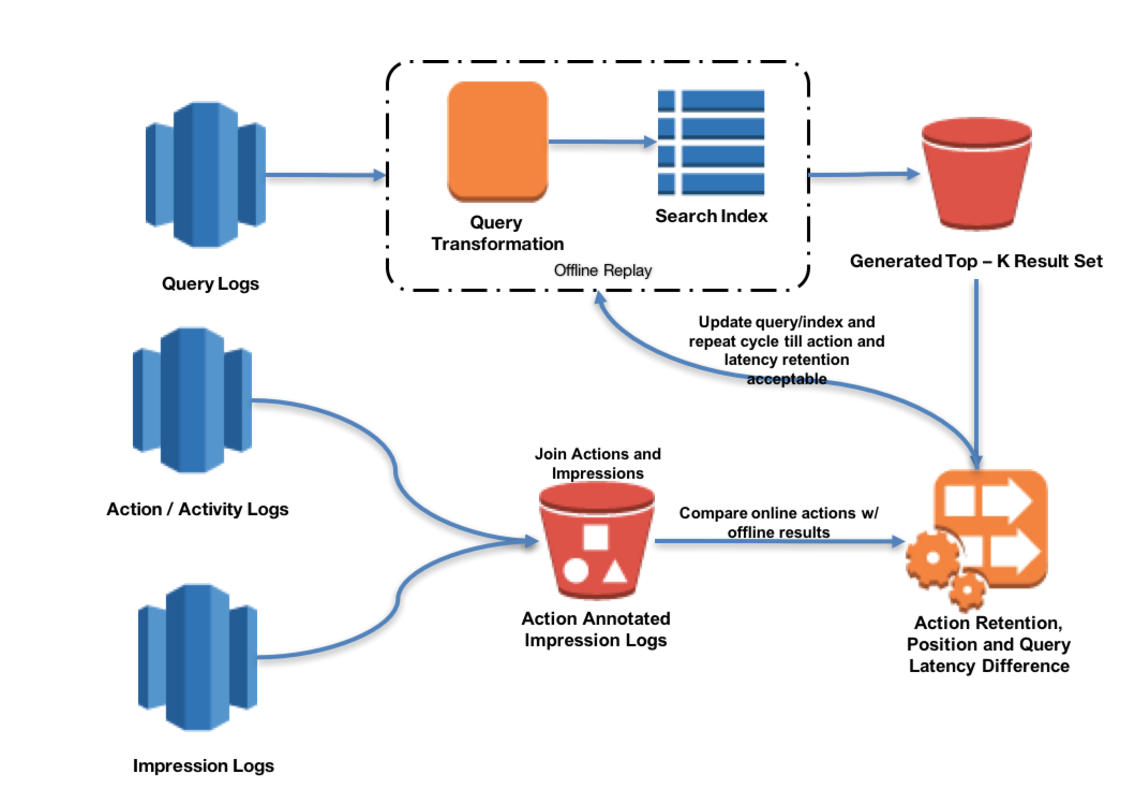
\includegraphics[width=\textwidth,scale=0.50]{replay-architecture.png}
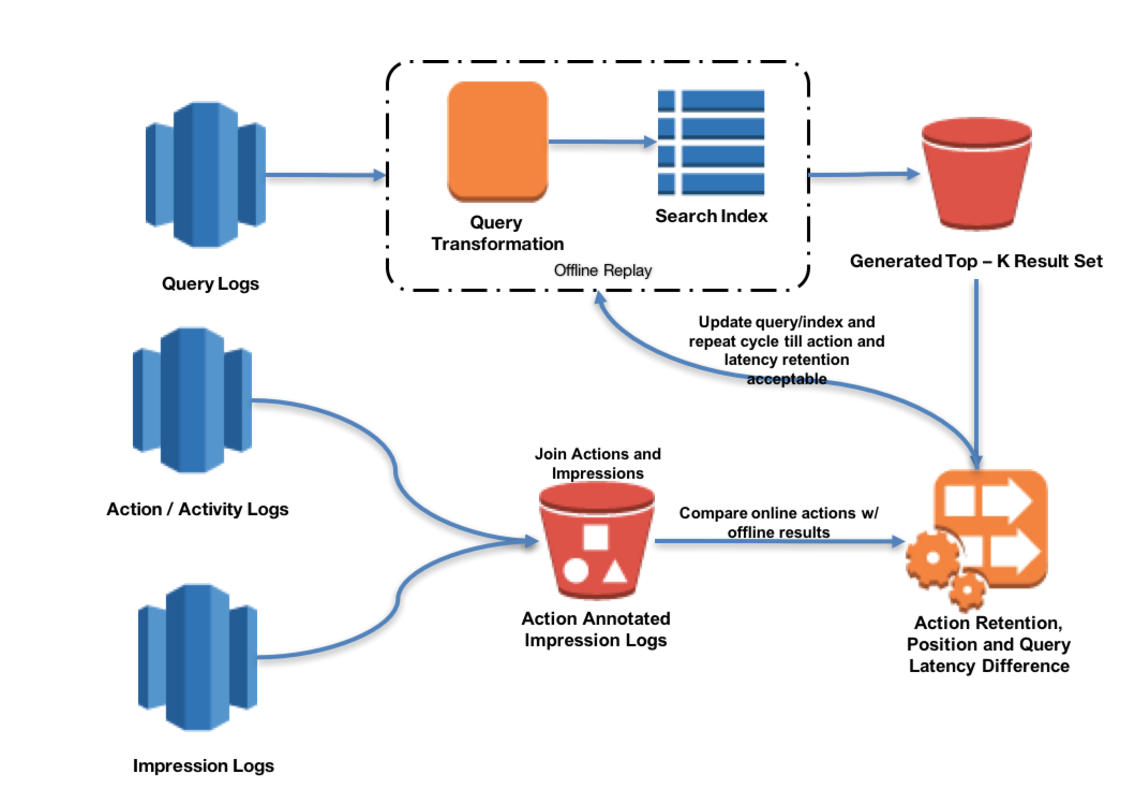
\includegraphics[scale=0.90]{replay-architecture.png}
\caption{Replay Framework}
\label{fig:replay-architecture}
\end{figure*}

At the core of the query construction process is an offline replay framework
shown in Figure~[\ref{fig:replay-architecture}]. This helps us in validating how we 
are doing compared to the baseline candidate selection model as well as to only 
take the best and validated queries to production.
We document the individual components that are part of the replay cycle and show 
examples from job recommendations vertical.

\subsubsection{Query, Impression and Activity Tracking}

For the replay of the queries we require support to track the query that 
was done online along with the results that were retrieved, ranked and 
shown to the members and guests. The tracking requires the exact retrieval 
query to be tracked. 
The exact query allows us to make modifications to query construction 
and use the same in the replay framework. This removes the need 
for regenerating the query with all member and job features and be sure 
what query was used to generate the tracked results. 

The tracked results are annotated with the specific actions that are needed 
for evaluation in the replay framework. As an example, in case of job 
recommendations we track job views and applications, and dismiss actions 
for each of the tracked job recommendations. 

\subsubsection{Offline Replay}
The offline replay can be broken down into the following steps: 
\begin{itemize}
\item Online data aggregation
\item Query log preparation
\item Query log replay
\item Analysis of replay results 
\end{itemize}

It utilizes the online query logs and runs a transformation to allow operations such as
query construction, replaying ranking with particular models etc.

The original queries are parsed through the query transformer and 
new candidate selection model is added into the query config. 
As the next step, we take both the modified queries as well as the original 
queries and replay them on hadoop using offline retrieval infrastructure (known
as {\bf offline Galene})

The results collected through the replay are then passed to a result 
comparator which goes through both the baseline and new rank-list and 
computes the action retention metrics. As an example, in the case of job 
recommendations we compute. 
\begin{itemize}
\item Job View/Application/Dismiss Retention
\item Number of hits scored
\end{itemize}

As an additional step, we also compute the difference between the baseline and 
modified queries to see what jobs that had actions were missed. 
This allows us to revisit the candidate selection model to debug why we 
missed retrieving the jobs. 

The workflow is implemented in a generic manner 
in Hadoop and can be utilized for tasks outside of query construction such 
as training data generation, model validation and rank-list metrics computation. 


\begin{figure}
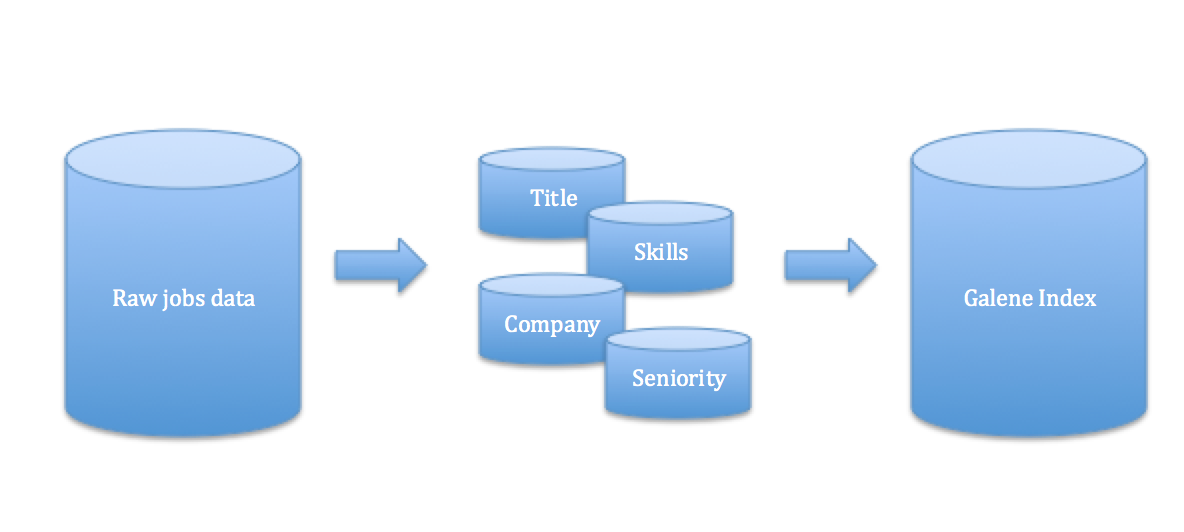
\includegraphics[width=\linewidth,height=\textheight,keepaspectratio]{offline-indexing.png}
\caption{Offline Indexing}
\label{fig:offline-indexing}
\end{figure}




\section{Query Construction Algorithm}

\begin{figure*}
\centering
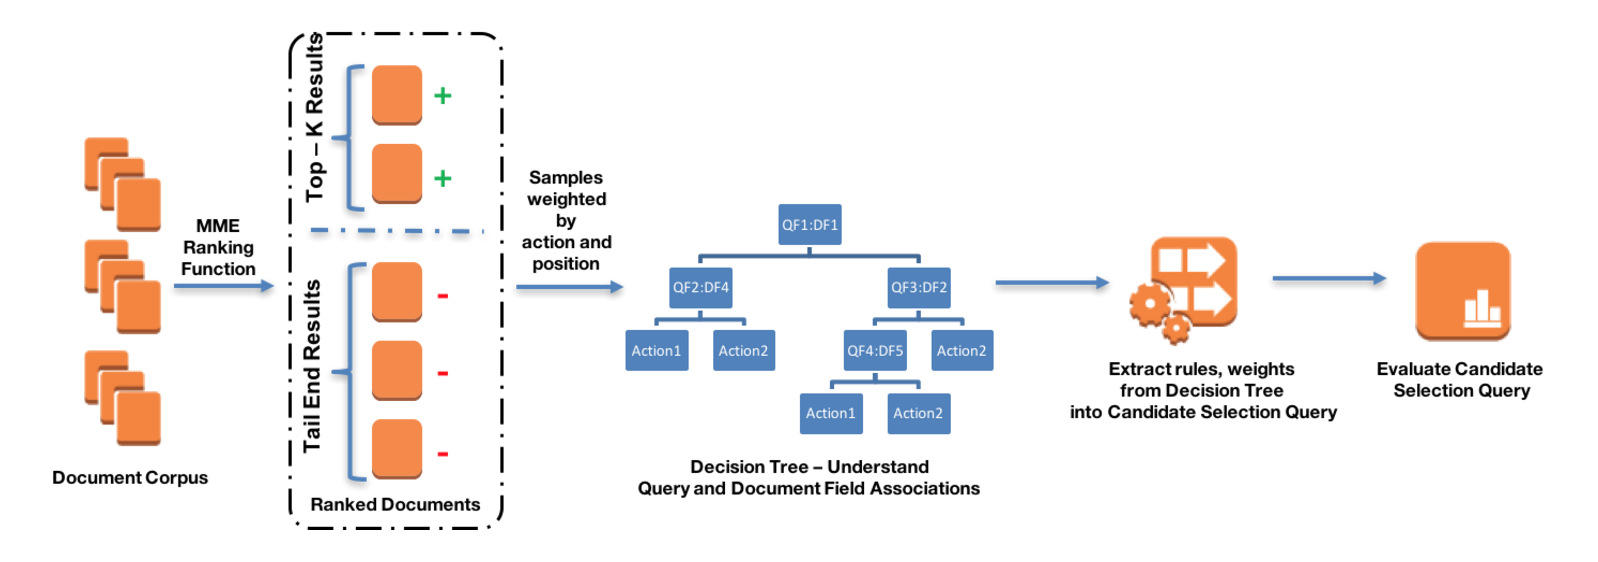
\includegraphics[width=\textwidth]{training-process.png}
\caption{Offline Training Process}
\label{fig:offline-training-process}
\end{figure*}


In this section, we describe the core algorithm used for query construction.
The entire flow is depicted in Figure~\ref{fig:offline-training-process} and
detailed below.
The algorithm consists of two steps:
\begin{enumerate}
    \item Construct decision tree using offline replay data
    \item Convert the decision tree into query clauses with weights. These
    weights will then be used in the WAND operators described in Section~[\ref{sec:wand}].
\end{enumerate}

The process of constructing decision trees and extracting clauses can be iterative. The depth of the decision tree is a hyper
parameter which can be tuned based on the output of the clauses. We will
describe details in this section.

\subsection{Decision Tree Construction}

The decision tree construction which in turn can be used for query
construction is described in Algorithm~\ref{alg:decision-tree2}. The branching
variables in the decision trees are all features described below. Consider $J_f$ 
and $M_f$ to be relevant fields in job details
and member profiles respectively. All {\it cross matches} in $J_f \times M_f$ are
potentially cross features which can be used as query clauses as well as
branching points in decision trees. Example, consider field in the job called
{\it Job Title} and a member profile field called {\bf Member Current Title}, a
potential feature would be {\it Job Title matches member current title}. Other
similar examples include:
\begin{enumerate}
    \item Job location matches member profile location
    \item Job company size matches member preference for company size
\end{enumerate}
Let $F$ represent the cumulative set of such features. We first sample set of
queries from production (say $Q$). We then run each query in this set through
our offline replay framework. Offline replay ranks the document set as well as
extracts the value of features in the feature set $F$. Assuming that the
original ranking is not bad (a reasonable assumption), we could use the top
$k_1$ results as positive and bottom $k_2$ as negative. We then have a dataset
of features and labels which can be run through pretty much any decision tree
based algorithm~\cite{quinlan1986induction} to extract a tree. 


\begin{algorithm}
\caption{Decision Tree Construction}\label{alg:decision-tree2}
\begin{algorithmic}[1]
  \State \textbf{Input}: User and query logs with queries, member activity, member profile and job
  details.
  \State \textbf{Output}: Decision tree Graph $G(V, E)$.
  $v \in V$ represents a feature, edge $e \in E$ to be represented by the tuple
  $(u, v, d, w)$ where $(u, v)$ represent nodes, $d$ represents the decision
  and $w$ represents the weight.
  \State Derive feature set $F$ which consists of cross query level cross
  features between job details and member profiles
  \State Sample queries from production into query set $Q$
  \State $T \gets \emptyset$
  \For {query $q \in Q$}
    \State Generate top $K$ results
    \State Extract features for each result
    \State Mark top $k_1$ results as positives $P$
    \State Mark bottom $k_2$ results as negatives $N$
    \State $T \gets T \cup P \cup N$
  \EndFor
  \State Run any standard decision tree algorithm on training set $T$ to get
  decision tree graph $G(V, E)$. 
  \State Use entropy at the decision tree edges to derive weight of each edge.
  \State %newline
\end{algorithmic}
\end{algorithm}

\subsection{Query Construction}

The entire to construct the queries is shown in
Algorithm~\ref{alg:query-construction}. The input to the algorithm is query
logs and some hyper parameters. These hyper parameters control the depth of the
tree as well as the number of positive and negative labels needed to get an
appropriate query clause. Like any decision tree, we expect to know the number
of positive and negative labels at each leaf node. The algorithm goes through a
loop terminating when a suitable solution is found or maximum tree depth is
reached. We start with min depth and construct a decision tree. Once the tree
is constructed, we enumerate all paths and cut off at a point when the number of
positive samples (at leaf nodes of each path) is more than a certain fraction
of the total positives. We also need to make sure that the number of negative
samples is low enough. If the constraint for both positive and negative samples
is met, we stop and return the path. If not, we try to build a deeper tree.

To give a general idea of how the queries are constructed we can look at a sample decision tree in Figure ~\ref{fig:decision-tree}.
Let us assume total positive coverage $\alpha$ is $0.06$ and hyper parameter $\beta$ is $0.04$. We describe the query construction in the following steps: 

\begin{enumerate}
    \item Let's say we have a member $M$ with following fields:
    \begin{itemize}
    \item Current Title = Software Engineer
    \item Member Seniority = Entry Level
    \item Member skill = Computer Science
    \end{itemize}
    \item We use standard depth first search on our decision tree to extract all the paths starting from root to leaf. We will refer to this set as $S_c$.
    \item $S_c$ is then sorted by number of positives labels that each path holds. We define the number of positives in a set by $P_+$ and number of negatives by $P_-$
    \item We iterate over the set $S_c$ to find a subset $S_c'$ which satisfy the constraint that $P_+'$ is greater $\alpha * P_+$ and $\frac{numNegativeLabels(P_{-})}{numPositiveLabels(P_{+})} \leq \beta$. 
    \item In our example, the paths indicated in green color satisfies the above constraints, since $P_+'= 5000$  is greater than $P_+ * \alpha = 4320$ and  $P'_-/P'_+ = 0.03 \leq \beta$
    \item All the paths in subset $S_c'$ can then be constructed as a OR Lucene query~\cite{mccandless2010lucene} where each path is an AND of features. In our example we have total four paths starting from root to leaf and only two paths marked in green color satisfy the constraints. Constructed query $CQ$ formed  using set of all valid paths $S_c'$ and  a member $M$ will look like the following: 
    \begin{itemize}
    \item \lucenequery{+(?(+jobTitle:Software Engineer +jobSkill: Computer Science) ?(+jobTitle:Software Engineer -jobSkill:Computer Science))}
    \end{itemize}
    \item The entropy measure at each node can be used directly to get the
        weights if we need to use a WAND query
    
\end{enumerate}

\begin{algorithm}
\caption{Query Construction}\label{alg:query-construction}
\begin{algorithmic}[1]

    \State \textbf{Input}: Query logs $Q_l$ with member activities, job details
    and member profile. $\alpha$ hyper parameters representing
    percentage of positives we want to cover. $\beta$ hyper parameter
    representing the min ratio of positives to negatives. $h_{max}$ and $h_{min}$ represent
    the maximum and minimum depth of the decision tree respectively.
    \State \textbf{Output}: Query clauses for search or recommendations
    \Function{constructClauses}{$\alpha$, $\beta$, $h_{max}$} 
        \State $h$ $\gets$ $h_{min}$
        \While {True}
            \State $G(V,E) \gets \Call{decisionTreeLearner}{Q_l, h}$
            \State $P \gets allPaths(G)$
            \State Sort $P$ by numPositiveLabels
            \State $P_{+} \subseteq P$ such that numPositiveLabels($P_+$) $\geq \alpha * numPositiveLabels(P)$
            \State 
            %\If{$\frac{numPositiveLabels(P_+)}{numNegativeLabels(P_{_})} \geq \beta$ or $h \geq h_{max}$}
            \If{$h \geq h_{max}$ or $\frac{numNegativeLabels(P_{-})}{numPositiveLabels(P_{+})} \leq \beta$}
                \State break     
            \EndIf
            $h \gets h + 1$
            \State 
        \EndWhile
        Clauses = extractClauses($P_+$)

    \EndFunction

\end{algorithmic}
\end{algorithm}



\begin{figure*}
\centering
    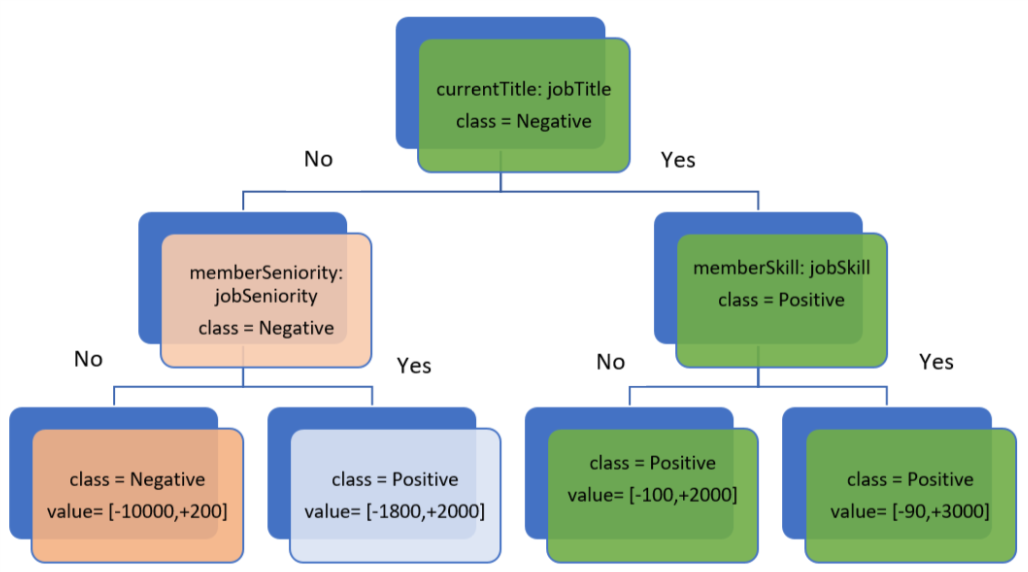
\includegraphics[width=\textwidth]{decision-tree-final.png}
\caption{Decision Tree}
\label{fig:decision-tree}
\end{figure*}



\section{Experiments}
In this section, we describe the experimental results using the proposed query
construction techniques. We used the techniques to run on two separate products
- job search and recommendations. We present the effectiveness in latency
reduction as well as quality. 

\subsection{Experimental Setup}
As mentioned in Section~[\ref{sec:system-architecture}], our underlying
retrieval is powered by an inverted index. We have two separate indices for
both job search and recommendations. The data required to train our models is
stored in HDFS. Our training pipeline is written using a combination of tools
including Apache Spark~\cite{meng2016mllib} and Photon~\cite{XianXing2016}. 

Our entire experimentation process consists of the following steps:
\begin{enumerate}
        \item Come up with query construction using techniques described
            earlier
        \item Measure impact offline using the replay framework
        \item Launch it online for a small percentage of population
        \item Retrain underlying ranking model using the results from new query
            construction
        \item Launch model online with new query construction and retrained
            ranking model
\end{enumerate}

We had two types of experiments - offline and online. Offline experimentation
uses the framework described in Section~\ref{sec:replay-framework}. In this
framework, we have ways to run a representative sample of production queries
through the new and old query construction. 
All
online experiments were conducted using LinkedIn's A/B testing 
framework~\cite{xu2015infrastructure}.

Retraining the underlying ranking models is done via our model training flow
details about which can be found in~\cite{zhang2016glmix} and~\cite{liget} for
jobs recommendations and search respectively. We use user actions to infer
labels in our models. These include:
\begin{itemize}
        \item Job clicks
        \item Job applies (typically stronger intent)
        \item Job dismisses. Our UI allows a user to dismiss a job from our
            jobs home page. This is generally signal for poor match
\end{itemize}

%Job search has a separate model and feature sets. In the presence of an
%explicit user query, we could build query to document features as well as
%features based on query understanding. We infer labels from user actions and
%use coordinate ascent to optimize a listwise ranking function~\cite{metzler2007linear}. 

\subsection{Jobs Recommendations}


Offline replay framework was used to sample a bunch of queries from the query
log and ran it through two different systems - one that uses old query
formulation and another one that uses the new proposed technique. 
We use the framework to train the decision trees as described in Section 5.  

For jobs recommendations, we use above labels inferred from member activities 
to build a deeply personalized
model. The objective of the model is to predict if a member $m$ will apply for
a job $j$ in context $t$. Let $q_m$ and $s_j$ denote the feature vector 
extracted from the member profile $m$ and job $j$ respectively. Let $x_{mjt}$
represent the overall feature vector for the the $(m, j, t)$ tuple. We use
logistic regression to predict the likelihood of member applying to job by:
\begin{equation} \label{eqn:glmix}
    g(E[y_{mjt}]) = x^{T}b + s^{T}_{j}\alpha_{m} + q^{T}_{m}\beta_{j}
\end{equation}
In the above equation:
\begin{itemize}
        \item $g(x) = log\frac{x}{1-x}$.
        \item  $b$ represents the global coefficient vector or simple the {\it
            global model}.
        \item $\alpha_m$ and $\beta_j$ are the coefficient vectors of member
            $m$ and job $j$ respectively. These coefficients are also called as
            random effects coefficients and enable deep personalization.

\end{itemize}
The details of the ranking model can be found in~\cite{zhang2016glmix}. Once we
obtain a decision tree, we retrain the model from activity data obtained from
the new model. This process is critical for both search and recommendations. We
have noticed that changing query formulation often requires us to retrain the
underlying ranking model. Note that we haven't changed anything in the ranking
model, but only retrained it using new data.

The main goal of the work is to reduce latency. Within latency, we
measure average, p95 (which represents the worst 5\% of queries) and p99 (worst
1\% of queries). Operational requirements are dictated more via the worst
queries than average case and hence the need to measure p95/p99

Table~[\ref{tab:jymbii-latency}] gives the p99 latency reduction while running
our decision tree based approach. The baseline approach we used was also a
machine learned algorithm described in~\cite{borisyuk2016casmos}.
As seen from the table, we notice significant reduction in latencies across the
spectrum. Note that these numbers were obtained by A/B testing online with a
sample of users directed to the new query construction techniques. These are
true latencies measured in our backend servers. Of particular interest in the
performance on the worst 1\% of the queries where we reduced latency by over
55\%. Average latencies were down by 35.6\%.

\TODO{write stuff about feed}

\begin{table*}
\centering
\caption{Impact of Query Construction on Jobs Recommendations Latency}
\begin{tabular}{|l|l|l|l|} \hline
Metric&Baseline&Decision Trees&Percentage Difference \\ \hline
Average Latency& 37.67 ms&24.26  ms& \bf{-35.6\%} \\ \hline
p95 latency& 163.2 ms& 109.9 ms& \bf{-48.49\%} \\ \hline
p99 latency& 562.4 ms&247.7  ms& \bf{-55.96\%} \\ \hline
\end{tabular}
\label{tab:jymbii-latency}
\end{table*}

\subsection{Job Search Experiments}

As with jobs recommendations, we employed the same query construction framework
with job search. Search also has an explcit query and facets from the user
which have to be incorporated as part of the query. For example, if a user
query is {\it ``marketing''} we could rewrite the query as:

\lucenequery{+(?TITLE:marketing ?SKILL:marketing)}

The above query may still be broad. Suppose we know from the users profile and
activities that the user is only interested in jobs from San Francisco,
California (represented as $SF-CA-USA$), we could rewrite the query as:

\lucenequery{+(?TITLE:marketing ?SKILL:marketing) +GEO:SF-CA-USA}

Such query rewriting reduces the number of documents ranked while maintaining
the precision. The underlying ranking model optimizes NDCG@K using inferred
labels from member activities~\cite{liget}. We perform top K randomization for
a very small percentage of production traffic. This randomization takes care of
position bias. The process followed then is similar to that of recommendations.
We run the constructed query through small sample of production traffic,
collect unbiased data, retrain the ranking model and put it back in production
for A/B testing.


Table~[\ref{tab:jobsearch-latency}] gives the latency reduction in job search
while deploying our query construction techniques. Unlike recommendations, 
job search has an explicit query which by itself can reduce the number of documents ranked.
However we do see some broad queries which can have very long latency. 
Hence the impact of the changes on p99 were much more pronounced. p99 went down
by {\bf 67.72\%}. 

\begin{table*}
\centering
\caption{Impact of Query Construction on Job Search Latency}
\begin{tabular}{|l|l|l|l|} \hline
Metric&Baseline&Decision Trees&Percentage Difference \\ \hline
Average Latency& 108.0 ms& 101.0  ms& \bf{-6.48\%} \\ \hline
p95 latency& 629 ms& 214  ms& \bf{-34.55\%} \\ \hline
p99 latency& 1921 ms&620  ms& \bf{-67.72\%} \\ \hline
\end{tabular}
\label{tab:jobsearch-latency}
\end{table*}

\section{Deployment Lessons}

When we changed the query construction, our first set of experiments were not
successful. While debugging the issue, we found that ranking also changed
significantly. This is due to the fact that the underlying model was trained on
data generated by the a different query construction. We then retrained our
model and found it to be successful. Whenever we change pre retrieval stage
significantly, we need to retrain the model. This pattern has been observed
repeatedly.

Biases in training data can also play a significant role in overall model
quality. We perform top K randomization and measure our offline models in job
search againts this data. We have found tigher correlation between offline and
online metrics by using unbiased data.

\section{Conclusions}
In this paper, we proposed a decision tree based method for query construction
targeted at job search and recommendations at LinkedIn. We detailed techniques
to convert member activities and query logs into query clauses. These query cl

In this work, we detailed techniques used to solve the query construction problem 
via decision trees. We developed an offline replay framework which can be
leveraged to construct a decision tree based on query logs and member
activities. We developed an algorithm to convert the decision tree into query
clauses. These query clauses can be used to construct an efficient search or
recommendations query. Such a query construction helped us reduce the latency
by over {\bf 67\%} while maintaining the quality metrics. The techniques
detailed in this work has been A/B tested with live production traffic and has
been ramped to 100\% of LinkedIn users.


%\end{document}  % This is where a 'short' article might terminate

%
% The following two commands are all you need in the
% initial runs of your .tex file to
% produce the bibliography for the citations in your paper.
\bibliographystyle{abbrv}
\bibliography{sigproc}  % sigproc.bib is the name of the Bibliography in this case
% You must have a proper ".bib" file
%  and remember to run:
% latex bibtex latex latex
% to resolve all references
%
% ACM needs 'a single self-contained file'!
%
%APPENDICES are optional
%\balancecolumns
% This next section command marks the start of
% Appendix B, and does not continue the present hierarchy
%\balancecolumns % GM June 2007
% That's all folks!
% This is "sig-alternate.tex" V2.1 April 2013
% This file should be compiled with V2.5 of "sig-alternate.cls" May 2012
%
% This example file demonstrates the use of the 'sig-alternate.cls'
% V2.5 LaTeX2e document class file. It is for those submitting
% articles to ACM Conference Proceedings WHO DO NOT WISH TO
% STRICTLY ADHERE TO THE SIGS (PUBS-BOARD-ENDORSED) STYLE.
% The 'sig-alternate.cls' file will produce a similar-looking,
% albeit, 'tighter' paper resulting in, invariably, fewer pages.
%
% ----------------------------------------------------------------------------------------------------------------

%\end{document}  % This is where a 'short' article might terminate

%
% The following two commands are all you need in the
% initial runs of your .tex file to
% produce the bibliography for the citations in your paper.
% You must have a proper ".bib" file
%  and remember to run:
% latex bibtex latex latex
% to resolve all references
%
% ACM needs 'a single self-contained file'!
%
%APPENDICES are optional
%\balancecolumns
% This next section command marks the start of
% Appendix B, and does not continue the present hierarchy
%\balancecolumns % GM June 2007
% That's all folks!
\end{document}
